%%%%%%%%%%%%%%%%%%%%%%%%%%%%%%%%%%%%%%%%%%%%%%%%%%%%%%%%%%%%%%%
\section{Muons}\label{sec:muons}
%%%%%%%%%%%%%%%%%%%%%%%%%%%%%%%%%%%%%%%%%%%%%%%%%%%%%%%%%%%%%%%

%%%%%%%%
\subsection{Muon reconstruction}
%%%%%%%%

The CMS detector is specifically designed for the optimization of muon detection, as its name clearly states. 
%Indeed the detection and high precision measurement of muons play key roles in many physics processes of interest such as the ones described in this thesis.
%The detection and high precision measurement of muons is very important for CMS. Many processes of interest involve muons in their final states, like the Higgs decay channel H$\rightarrow$ZZ$\rightarrow$4$\mu$ . In fact, CMS is specifically designed for the optimization of muon detection, as its name clearly states.
In general, muons will not be absorbed by the calorimeters, as is what happens with electrons, so a specific muon detection system (Section~\ref{subsec:muonchambers}) is needed in order to identify them.\\
%and improve the resolution of their momenta as measured by the tracking system.\\

In the standard CMS reconstruction~\cite{Chatrchyan:2012xi}, tracks are first reconstructed independently in the inner tracker (tracker track) and in the muon system (standalone-muon track).
%Based on these objects, two reconstruction approaches are used:
A standalone-muon track is reconstructed from pre-built track segments (i.e. a set of aligned DT or CSC hits) in the muon chambers. The state vector associated to the segments found in the innermost chambers is used to seed the muon trajectory, from inside out, using the KF technique: the predicted state vector at the next measurement surface is compared with existing hits and updated accordingly. A suitable $\chi^2$ cut is applied to reject bad hits and the procedure is iterated until the outermost surface of the muon system is reached. Finally, the track is extrapolated to the nominal interaction point and a vertex-constrained fit is performed. The magnetic field, the multiple scattering inside the steel yoke, and the energy loses are taken into account.

Based on reconstructed standalone-muon and tracker tracks, two reconstruction approaches are then used:

\begin{itemize}
\item {\bf global-muon reconstruction (outside-in)}: each standalone-muon track is extrapolated to the tracker and a search is performed in a cone around it to match a tracker track; a global-muon track is fit combining hits from the tracker track and standalone-muon track, using the KF technique;
\item {\bf tracker-muon reconstruction (inside-out)}: all tracker tracks with $\pt > 0.5\GeV$ are considered as possible muon candidates and are extrapolated to the muon system while searching for a match with at least one muon segment.
\end{itemize}

Tracker-muon reconstruction is more efficient than the global-muon reconstruction at low momenta, $\pt \leq$ 5\GeV, because it requires only a single muon segment in the muon system, whereas global-muon reconstruction is designed to have high efficiency for muons penetrating through more than one muon station, and typically requires segments in at least two muon stations. However, given the high efficiency of both the tracker track and muon segments reconstruction, about 99\% of muons produced within the geometrical acceptance of the muon system and having sufficiently high momentum ($\pt \geq$ 5\GeV) are reconstructed by both methods. As shown in Fig.~\ref{fig:mu_ptrel} the additional information provided by the muon system is precious for the momentum reconstruction of high-energy muons ($\pt \geq$ 200\GeV), for which the tracker-only momentum measurement is degraded. 
In fact, as a particle's momentum increases and the curvature of its corresponding track decreases, the momentum resolution in the tracker becomes limited by position measurement resolution. One can then benefit from the large lever arm and 3.8\unit{T} magnetic field in the region between the tracker and the muon system by including hits in the muon chambers. For lower momenta, instead, the resolution of the tracking system is dominating.
%At large transverse momenta, pT $\geq$ 200\GeV/c, the global-muon fit can improve the momentum resolution compared to the tracker-only fit.
%A tracker muon is less restrictive in the muon system reconstruction (only requires a muon segment) so it will be slightly more efficient for low-pT muons, which might not cross enough muon stations as to reconstruct a standalone track. 

\begin{figure}[!htb]
\centering
\subfigure[]{\hspace{-0.7cm}\label{fig:mu_ptrel_a}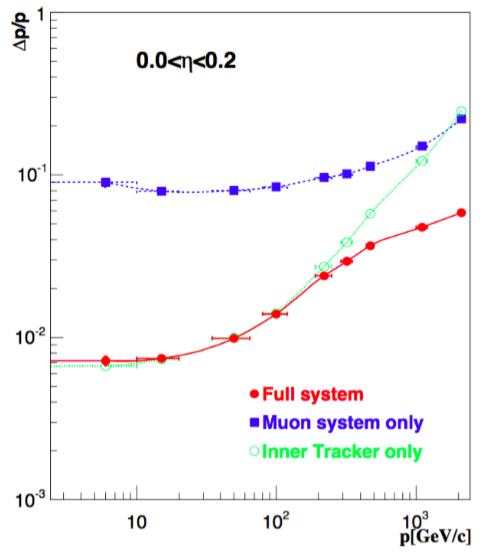
\includegraphics[width=0.38\textwidth]{\chsix/muon-pt-resolution-etabin0.png}}\quad\quad\quad
\subfigure[]{\hspace{-0.7cm}\label{fig:mu_ptrel_b}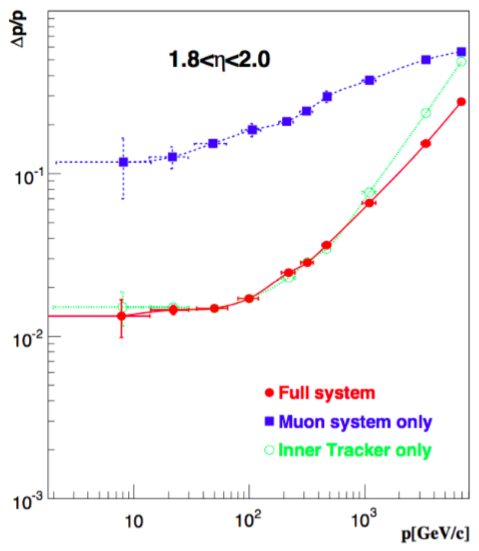
\includegraphics[width=0.38\textwidth]{\chsix/muon-pt-resolution-etabin1.png}}
\caption{Relative resolution of the muon momentum measurement for the reconstruction with the inner tracker only, the muon system only and for the combination of the inner tracker and the muon system, for simulated muons emitted in the central (a) and forward (b) regions~\cite{Bayatian:922757}.}
\label{fig:mu_ptrel}
\end{figure}

Figure~\ref{fig:mu_reco_eff} shows the muon tracking efficiency as a function of the $\eta$ of the probe muon and the number of primary vertices for 13\TeV data and simulation, evaluated using the T\&P method described in Section~\ref{subsec:elereco}. In the region $|\eta| < 2.2$ and for events with number of reconstructed primary vertices lower than 25, the measured tracking efficiency for isolated muons is $> 99\%$ in both data and simulation. The efficiency is constant as a function of the number of vertices in the event, hence it does not depend on the pileup.\\

\begin{figure}[!htb]
\centering
\subfigure[]{\label{fig:mu_reco_eff_a}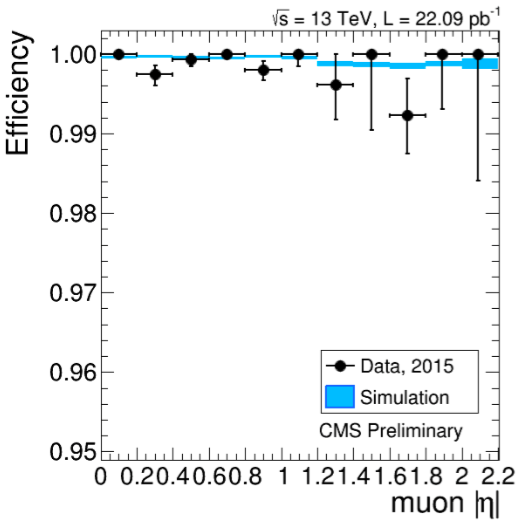
\includegraphics[width=0.38\textwidth]{\chsix/mu-reco-eff-eta.png}}
\subfigure[]{\label{fig:mu_reco_eff_b}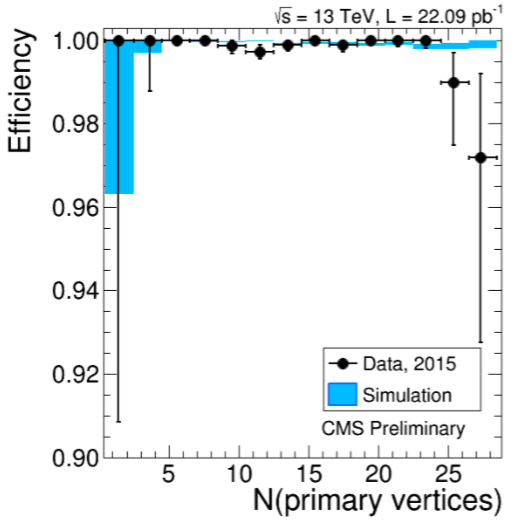
\includegraphics[width=0.38\textwidth]{\chsix/mu-reco-eff-PU.png}}
\caption{Tracking efficiency measured with a T\&P technique, for muons from Z decays, as a function of the muon $\eta$ (a) and the number of primary vertices (b), for 2015 data (black dots) and simulation (blue bands)~\cite{CMS-DP-2015-016}.}
\label{fig:mu_reco_eff}
\end{figure}

The combination of different algorithms provides robust and efficient muon reconstruction.
After the completion of both algorithms, the reconstructed stand-alone, global, and tracker muons are merged into a single software object, with the addition of further information, like isolation and energy collected in matching calorimeter towers. This information can be used for further identification, in order to achieve a balance between efficiency and purity of the muon sample as described in Section~\ref{subsec:muonid}.\\

The performance of the reconstruction for high-\pt muons is strongly affected by radiative processes and by the muon detector alignment. 
Electromagnetic showers and large energy losses can arise as the muon traverses the steel layers of the magnet return yoke, producing additional segments in the muon chambers.
These events can affect the measurement done in the muon detectors. Therefore, specialized reconstruction algorithms for high-\pt muons, known as ``TeV-muon'' refits, have been developed in CMS as described in the following.

The \textit{tracker-plus-first-muon-station} fit (TPFMS) only uses hits from the tracker and the innermost muon station with hits, to reduce the sensitivity to possible showering starting deeper in the muon system. The \textit{Picky} fit uses all tracker hits, while a selection is applied to muon hits. Hits from chambers with a high probability of shower contamination (determined from the hit occupancy) are required to be compatible with the extrapolated trajectory by applying a $\chi^2$ cut. The \textit{dynamic truncation} algorithm (DYT) starts from the idea that the muon track reconstruction should be stopped after a large energy loss, as hits produced after that can only bias the momentum measurement. For every global muon trajectory the algorithm starts from the corresponding tracker track and propagates it out to the muon stations. Compatible segments (or hits) in the muon chambers are found by using an estimator which takes into account the propagation of the tracker covariance matrix through the material and the magnetic field, and the covariance matrices of the candidate muon segments (or hits).

Momentum assignment is then performed by the \textit{Cocktail} algorithm which combines the above methods to further improve the resolution at high \pt reducing the tails of the momentum resolution distribution.
In particular, the algorithm chooses, on a track-by-track basis, the best muon reconstruction. For Run~1, the Cocktail-algorithm decision is taken between the tracker-only, TPFMS, and Picky fits. 
This version of the algorithm is also known as the \textit{Tune P} algorithm. It starts with the Picky fit, then switches to the tracker-only fit if the goodness of fit ($\chi^2$/n.d.f.) of the latter is significantly better. Then it compares the $\chi^2$/n.d.f. of the chosen track with that of TPFMS; TPFMS is chosen if it is found to be better. For high-\pt muons, TPFMS and Picky algorithms are selected by Tune P in most of the cases, in approximately equal amounts, while the tracker-only fit is selected only in a few percent of events. 

For Run~2, the Tune P algorithm was extended to include also the DYT fit. The selection is still made on a track-by-track basis, but using both the $\chi^2$/n.d.f. of the track and the relative error of the \pt measurement. The algorithm starts with the Picky fit, then switches to DYT if the DYT track has a lower relative \pt error. It then compares the $\chi^2$/n.d.f. of the chosen track with that of the tracker-only fit and picks tracker-only if its $\chi^2$/n.d.f. is significantly better. Then the $\chi^2$/n.d.f. of the chosen track and TPFMS are compared and the one giving the best result is kept. At the end, if the final candidate track has \pt lower than 200\GeV or the tracker-only \pt is lower than 200\GeV, the tracker-only track is selected.%The momentum resolution obtained with this new optimized version of the Tune P algorithm, reaches 5.9\% for muons with \pt in the range $700 < \pt < 2000\GeV$, as measured with cosmic-ray muon data~\cite{Radogna:2205870}.

The momentum resolution obtained with the Tune P algorithm for muons with \pt in the range $350 < \pt < 2000\GeV$ is found to be $\approx$ 6\%, as measured with cosmic-ray muon data~\cite{Chatrchyan:2012xi,Radogna:2205870}.

%Specialized algorithms for high-energy muon reconstruction, known as ?TeV-muon? refits, have been developed in CMS and the final momentum assignment is performed by the so called ?Cocktail? algorithm which chooses the best muon track candidate. These algorithms have been updated and tuned to optimize the performance in collisions at 13 TeV.
%To further improve the resolution at high \pt, mainly by reducing the tails of the momentum resolution distribution, combinations of the above can be used. In particular, the Tune P al- gorithm chooses, on a muon-by-muon basis, between the tracker-only, TPFMS, and Picky fits. The algorithm starts with the Picky fit, then switches to the tracker-only fit if the goodness of fit of the latter is significantly better. Then it compares the goodness of fit of the chosen track with that of TPFMS; TPFMS is chosen if it is found to be better. For high-pT muons, TPFMS and Picky algorithms are selected by Tune P in most of the cases, in approximately equal amounts, while the tracker-only fit is selected only in a few percent of events

%%%%%%%%
\subsection{Muon trigger}\label{subsec:mutrigger}
%%%%%%%%

The Level-1 muon trigger uses signals from all three CMS muon detector systems: DT, CSC, and RPC. It has a latency of 3.2\mus and reduces the rate of the readout of events with muon candidates
at the detector front-end electronics to a few kHz by applying selections on the estimated muon \pt and quality.
In the muon HLT, first a Level-1 trigger object is used as a seed to reconstruct a standalone-muon track in the muon system, leading to an improved \pt estimate. At this point, \pt threshold filters are applied to the standalone-muon (also called Level-2 muon). Then seeds in the inner tracker are generated in the region around the extrapolated Level-2 muon, and tracker tracks are reconstructed. If a successful match is made between a tracker track and the Level-2 muon, a global fit combining tracker and muon hits is performed, yielding a Level-3 muon track on which the final \pt requirements are applied. In this way, the rate of recorded inclusive muon events is reduced to a few tens of Hz. The average processing time of the HLT reconstruction is about 50\unit{ms}.

The L1 and HLT trigger used to collect the data analyzed in this thesis are listed in Tables~\ref{tab:triggMu8TeV} and~\ref{tab:triggMu13TeV} for the 8 and 13\TeV data analysis, respectively.
For both analyses the HLT used to select the events is the unprescaled single-muon trigger with the lowest \pt threshold that does not include muon isolation requirements. 
%Both analyses requires one muon candidate. The HLT used to select the events is the unprescaled single-muon trigger with the lowest \pt threshold that does not include muon isolation requirements.
In fact, although muons produced by the leptonic decay of a high-\pt W boson tend to be isolated, their high momentum enhances the production of electromagnetic showers, that can mimic a non-isolated muon candidate.
Therefore, only requirements on the muon \pt and $\eta$ are applied at this stage.
The efficiency of the L1 single-muon trigger with the 16\GeV threshold is shown in Fig.~\ref{fig:mu_L1trigg} as a function of the offline reconstructed muon \pt and $\eta$. In 2012 the efficiency for this trigger was greater than 90\%. A similar result is obtained in 2015.
%The efficiency at the plateau is 2% lower in 2012 with respect to 2011 due to an optimization aimed to reduce the single muon trigger rate by 50% which allowed to keep pT thresholds for 2012 running as low as the ones used for 2011. In both 2011 and 2012 the efficiency of the L1 single muon trigger was greater than 90%.

\begin{table}[!htb]
\centering
\caption{The L1 and HLT single-muon triggers used to collect the 8\TeV data analyzed in this thesis together with the imposed requirements on the muon candidate.}
\begin{tabular}{ l | c | c }
Trigger & Name & Selections\\
\hline
\hline
\multirow{3}{*}{Level 1} & \multirow{3}{*}{L1\_SingleMu16\_eta2p1}                 & 1 global muon with:\\ 
                                     &                                                                                   & \pt $>$ 16\GeV\\
                                     &                                                                                   & $|\eta| <$ 2.1\\
\hline
\multirow{3}{*}{HLT} & \multirow{3}{*}{HLT\_Mu40\_eta2p1} & 1 global muon with:\\
                                &                                                            & \pt $>$ 40\GeV\\
                                &                                                            & $|\eta| <$ 2.1\\
\hline 
\end{tabular}
\label{tab:triggMu8TeV}
\end{table}

\begin{table}[!htb]
\centering
\caption{The L1 and HLT single-muon triggers used to collect the 13 TeV data analyzed in this thesis together with the imposed requirements on the muon candidate.}
\begin{tabular}{ l | c | c }
Trigger & Name & Selections\\
\hline
\hline
\multirow{2}{*}{Level 1} & \multirow{2}{*}{L1\_SingleMu25}  & 1 global muon with:\\ 
                                     &                                                       & \pt $>$ 25\GeV\\
\hline
\multirow{3}{*}{HLT} & \multirow{3}{*}{HLT\_Mu45\_eta2p1} & 1 global muon with:\\
                                &                                                            & \pt $>$ 45\GeV\\
                                &                                                            & $|\eta| <$ 2.1\\
\hline 
\end{tabular}
\label{tab:triggMu13TeV}
\end{table}

\begin{figure}[!htb]
\centering
\subfigure[]{\label{fig:mu_L1trigg_a}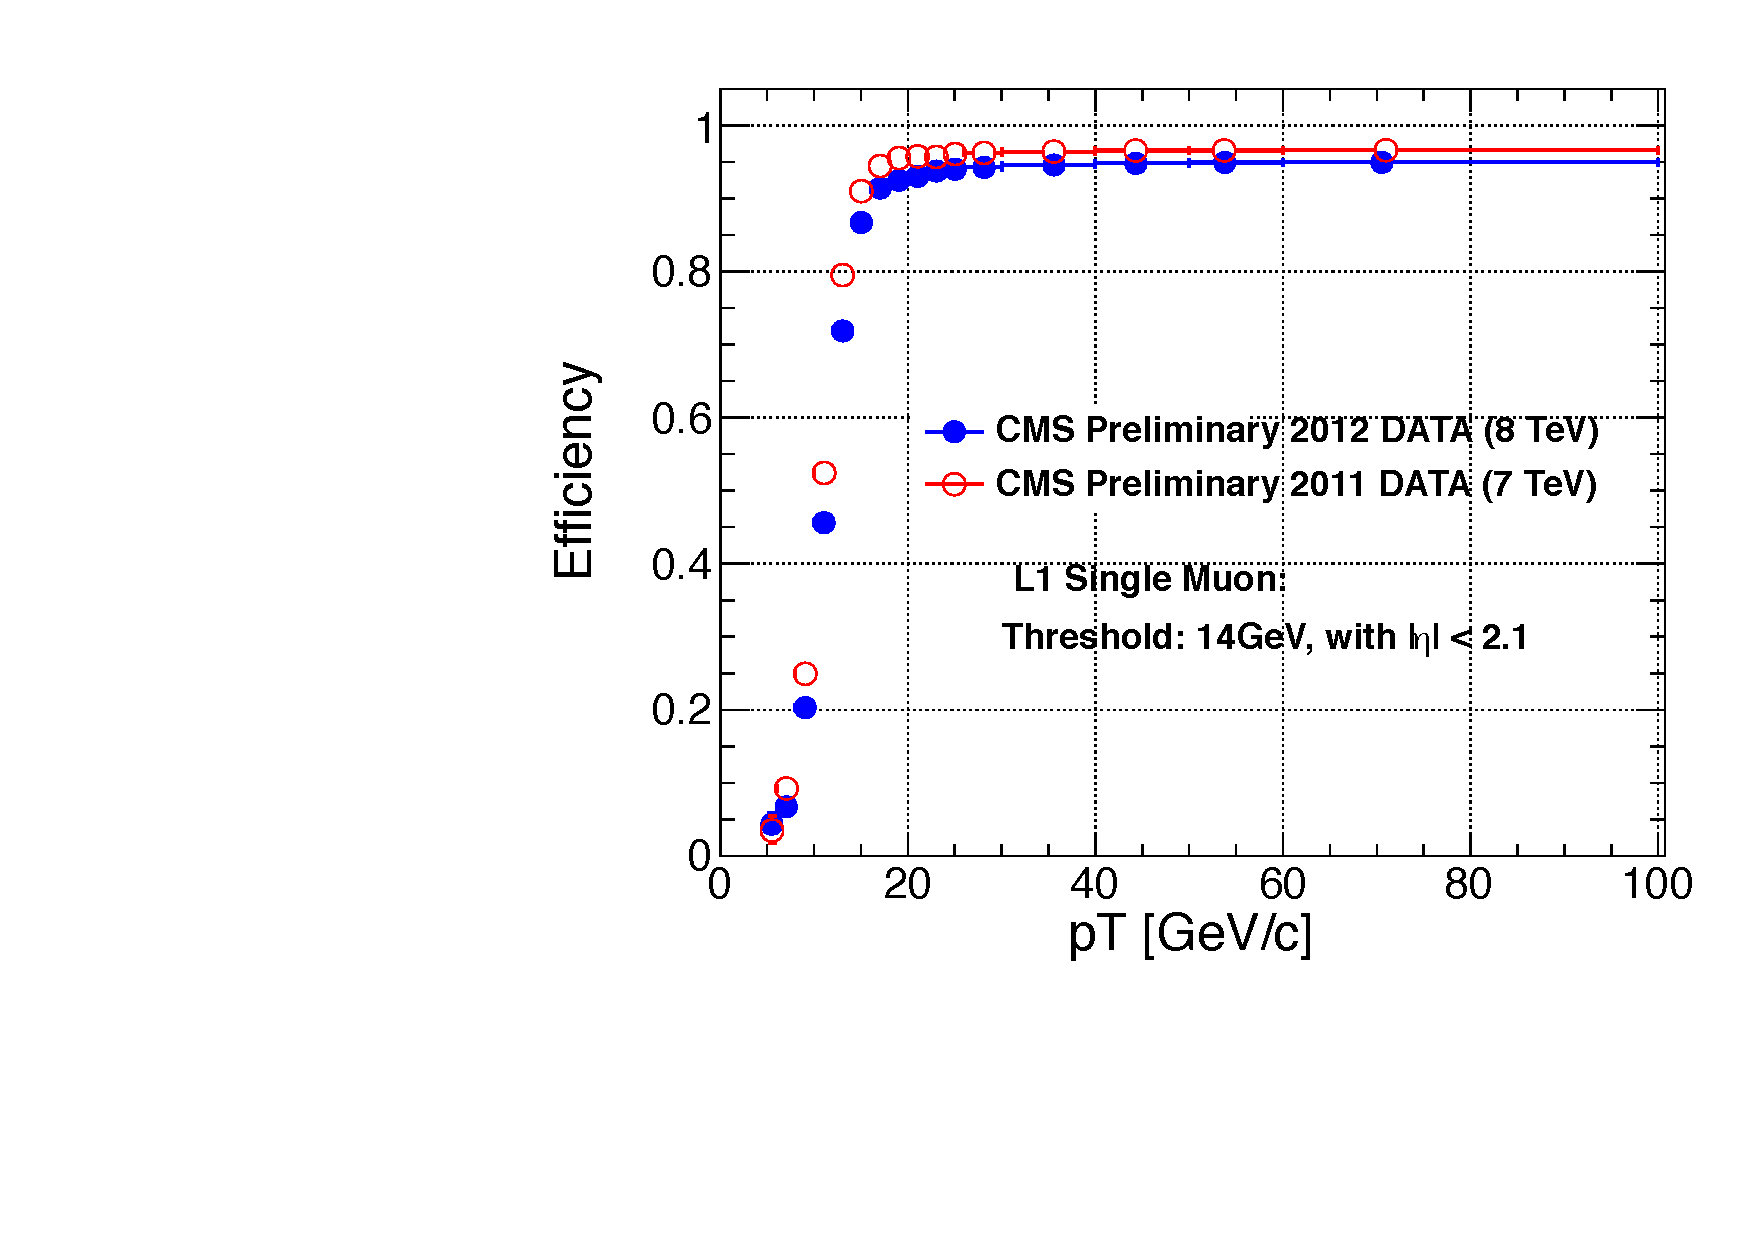
\includegraphics[width=0.45\textwidth]{\chsix/SingleMu16_pt.pdf}}
\subfigure[]{\label{fig:mu_L1trigg_b}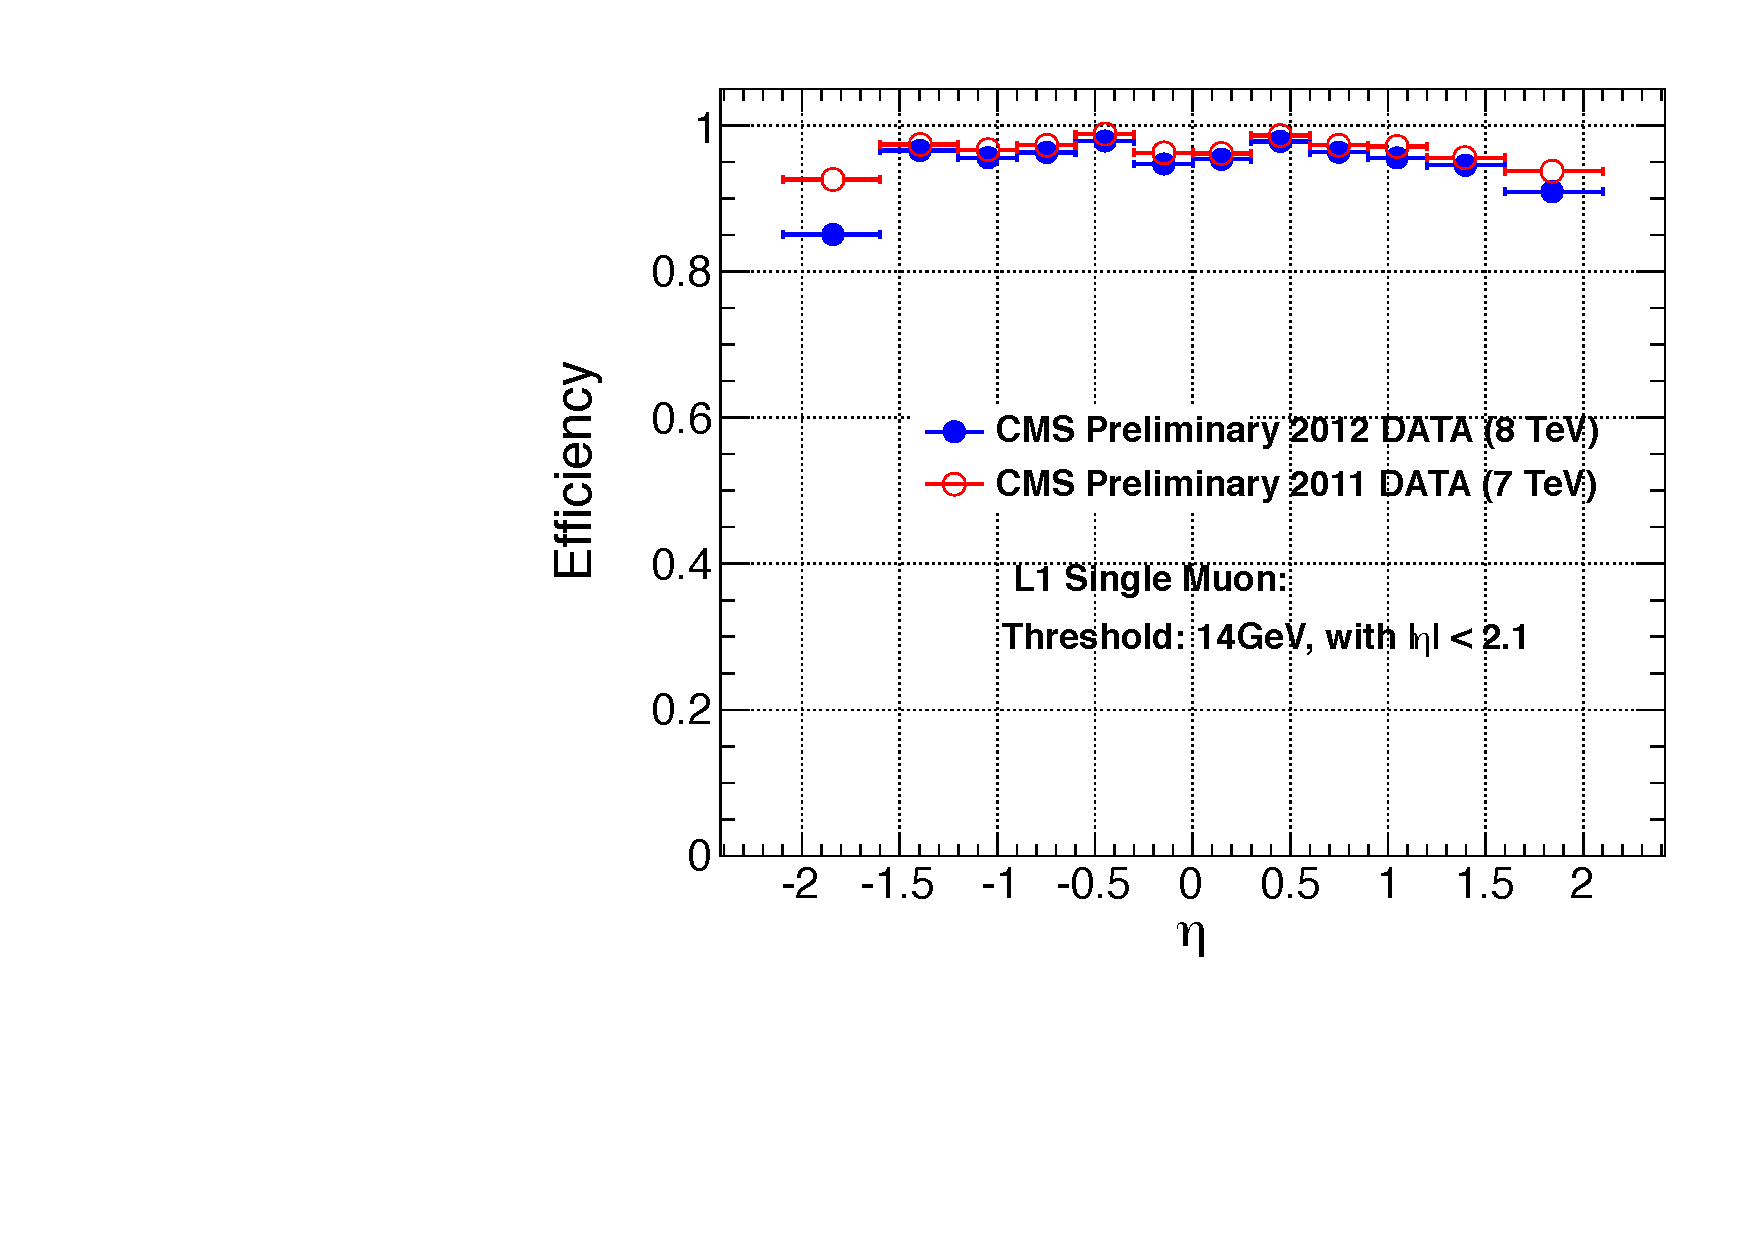
\includegraphics[width=0.45\textwidth]{\chsix/SingleMu16_eta.pdf}}
\caption{Efficiency of the L1 single-muon trigger with a threshold of 14\GeV on the muon \pt as a function of the muon \pt (a) and $\eta$ (b)~\cite{Brooke:1496888}.}
\label{fig:mu_L1trigg}
\end{figure}

%The offline reconstructed \pt of the muons must be greater than 50 (53) GeV for the 8 (13) TeV analysis, where the trigger reaches the plateau. Furthermore the selected muon must be reconstructed within $|\eta|$ < 2.1 as a consequence of the trigger criteria.
The efficiency for a muon passing the high-\pt selections described in Section~\ref{subsec:muonid} to fire the HLT single-muon triggers have been measured in data with T\&P method and are summarized in Tables~\ref{tab:hltMueff8TeV} and~\ref{tab:hltMueff13TeV}. 

\begin{table}[!htb]
\centering
\caption{Efficiencies and scale factors for the single-muon HLT trigger used in the 8\TeV analysis
for muons with \pt $>$ 50\GeV, $|\eta| <$ 2.1, and satisfying the high-\pt and isolation selections described in Section~\ref{subsec:muonid}.
The quoted uncertainties are statistical.}
\begin{tabular}{ c | c | c | c}
 & $0 < |\eta| < 0.9$ & $0.9 < |\eta| < 1.2$ & $1.2 < |\eta| < 2.1$\\
\hline
\hline
Efficiency simulation & 95.10\% $\pm$ 0.03\% & 87.01\% $\pm$ 0.03\% & 81.56\% $\pm$ 0.03\%\\
Efficiency data & 92.90\% $\pm$ 0.02\% & 83.14\% $\pm$ 0.06\% & 80.27\% $\pm$ 0.05\%\\
Data/simulation scale factor & 0.9768 $\pm$ 0.0004 & 0.956 $\pm$ 0.001 & 0.984 $\pm$ 0.001\\
\hline 
\end{tabular}
\label{tab:hltMueff8TeV}
\end{table}
%https://twiki.cern.ch/twiki/bin/viewauth/CMS/MuonReferenceEffs
%https://indico.cern.ch/event/257000/contributions/1586340/attachments/451105/625487/SingleMuTriggerEff_10June_updated.pdf

\begin{table}[!htb]
\centering
\caption{Efficiencies and scale factors for the single-muon HLT trigger used in the 13\TeV analysis
for muons with \pt $>$ 53\GeV, $|\eta| <$ 2.1, and satisfying the high-\pt and isolation selections described in Section~\ref{subsec:muonid}.
The quoted uncertainties are statistical.}
\begin{tabular}{ c | c | c | c}
 & $0 < |\eta| < 0.9$ & $0.9 < |\eta| < 1.2$ & $1.2 < |\eta| < 2.1$\\
\hline
\hline
Efficiency simulation & 97.6\% $\pm$ 0.1\% & 93.4\% $\pm$ 0.4\% & 94.8\% $\pm$ 0.2\%\\
Efficiency data & 94.6\% $\pm$ 0.2\% & 89.7\% $\pm$ 0.4\% & 91.8\% $\pm$ 0.2\%\\
Data/simulation scale factor & 0.969 $\pm$ 0.002 & 0.961 $\pm$ 0.006 & 0.968 $\pm$ 0.003\\
\hline 
\end{tabular}
\label{tab:hltMueff13TeV}
\end{table}
%https://twiki.cern.ch/twiki/bin/view/CMS/MuonReferenceEffsRun2
%https://indico.cern.ch/event/462268/contributions/1979019/attachments/1188638/1724574/2015.11.17_MuonPOG_SingleMuTrigEff_SF_KPLee_v2.pdf

%%%%%%%%
\subsection{Muon identification}\label{subsec:muonid}
%%%%%%%%

The standard CMS muon reconstruction provides additional information for each muon, useful for muon quality selection and identification in physics analyses~\cite{Chatrchyan:2012xi}. 
In general, particles detected as muons are produced in pp collision from different sources which lead to different experimental signatures. The so-called \textit{prompt muons} arise either from decays of W, Z, or promptly produced quarkonia states. Real muons are also produced in the decay of heavy flavour particles, such as beauty or charmed mesons, as well as in light hadron (pions or kaons) decays. Less frequently, muons might originate from a calorimeter shower or from a nuclear interaction in the detector. Furthermore, the so called ``punch-through'' effect, i.e. hadron shower remnants penetrating through the calorimeters and reaching the muon system, can lead to the reconstruction of a muon candidate. Most of the physics analyses in CMS studying SM processes or searching for BSM signals use prompt muons, while all the other categories of muons constitute the background. These analyses exploit the same set of information, although the applied selections might be different depending on the signature of interest and the expected background. In this section only the specific selection developed for high-\pt muons is described. One of the main difference with respect to the low- and medium-\pt muon selection is that this particular identification procedure does not use the PF algorithm. It is aimed at the best reconstruction of the muon track parameters without relying on external information on the event. Moreover, the goodness of the global-muon track fit selection, based on the $\chi^2$ of the track, is not requested, but an additional selection based on the relative \pt resolution for the track used for momentum determination is applied. 

The high-\pt muon selection criteria are described in the following and they have not been changed since Run~1:

\begin{itemize}
\item The muon must be reconstructed both as a tracker- and a global-muon. This is effective against decays-in-flight, punch-through and accidental matching (with noisy or background tracks or segments).
%\item The number of hits in the tracker track part of the muon. Generally tracks with small number of hits give bad pT estimate. In addition decays in flight give rise in many cases to lower hit occupancy in the tracks.
\item Number of pixel hits in the tracker track $\geq$ 1. To further suppress muons from decays in flight.
%\item There should be at least one pixel hit in the tracker track part of the muon. The innermost part of the tracker is an important handle to discard non-prompt muons. By requiring just a minimal number of hits we introduce negligible reconstruction inefficiency.
\item Number of tracker layers involved in the track measurement $\geq$ 6. This guarantees a good \pt measurement, for which some minimal number of measurement points in the tracker is needed. It also suppresses muons from decays in flight.
\item Number of muon-chamber hits included in the global-muon track fit $\geq$ 1. This requirement assures that the global muon is not an accidental match between the information from the muon system and the tracker. This could happen in particular for non-prompt muons or fake muons from punch-through.
%\item The global muon has to contain at least one ?valid? muon hit. This re- quirement assures that the global muon is not a ?bad? match between the information from the muon system and the tracker. This could happen in particular for non-prompt muons.
\item The muon track is required to have muon segments in at least 2 muon stations to further suppress punch-through and accidental track-to-segment matches. This selection is furthermore consistent with the logic of the single-muon trigger, which requires segments in at least two muon stations to obtain a meaningful estimate of the muon \pt.
%\item The muon track has to have a minimum number (2) of chamber hits in different stations with matching (consistent with the propagated to the muon chambers tracker track) segments. This is also to comply with a similar looser requirement in the trigger.
%\item Very bad fits are rejected by requiring reasonable global muon fit quality. If there is a decay in flight inside the tracking volume, the trajectory could contain a sizeable ?kink?, resulting in a poorer  2 of the fit used to determine the trajectory.
\item Transverse impact parameter of the muon track $< 2\mm$. This assures the compatibility of the muon track with the interaction point hypothesis and it is effective against cosmic background and further suppress muons from decays in flight.
\item Longitudinal impact parameter of the muon track $< 5\mm$. To further suppress cosmic muons, muons from decays in flight and tracks from pileup.
%\item Muon can be required also to be matched a Particle Flow (PF) muon. PF is a reconstruction technique widely used in CMS analyses. It makes use of the full detector information to describe the global collision event, by identifying particles individually and clustering them into more complex objects. More details about PF algorithm are available in [49,50].
\item Relative \pt error $< 30\%$. To further suppress mis-reconstructed muons.
\end{itemize}

In addition to these identification criteria, an isolation requirement is applied to the well-identified muons. In particular, the muon must pass a relative tracker-only isolation selection: the scalar sum of the \pt of all other tracks in a cone of  $\Delta R < 0.3$ around but not including the muon tracker track must be less than 10\% of the muon \pt, also as measured by the tracker. To be used in the calculation of the tracker-based isolation, tracks have to be within 2\mm, in the $z$ direction, of the primary vertex with which the muon candidate is associated. These additional criteria help suppress the effect of tracks originating from pileup on the reconstructed quantities.

The efficiency and data-to-simulation scale factors for the high-\pt muon identification and isolation criteria measured with the T\&P method in 8 and 13\TeV data are summarized, respectively, in Tables~\ref{tab:idMueff8TeV} and~\ref{tab:idMueff13TeV}. The scale factors are close to unity, indicating a good agreement between data and simulation. They are used in the analyses presented in this thesis to correct the normalization of simulations.

\begin{table}[!htb]
\centering
\caption{Efficiencies and scale factors for the high-\pt muon identification and isolation criteria used in the 8\TeV data analysis for muons with $\pt > 50\GeV$ and $|\eta| < 2.1$.}
\begin{tabular}{ l | c | c | c}
Muon $|\eta|$ & $0 < |\eta| < 0.9$ & $0.9 < |\eta| < 1.2$ & $1.2 < |\eta| < 2.1$\\
\hline
\hline
 & \multicolumn{3}{c}{High-\pt muon identification}\\
\hline
Efficiency simulation & 96.51\% $\pm$ 0.02\% & 96.61\% $\pm$ 0.04\% & 95.54\% $\pm$ 0.03\%\\
Efficiency data & 95.54\% $\pm$ 0.02\% & 95.87\% $\pm$ 0.04\% & 95.06\% $\pm$ 0.03\%\\
Data/simulation scale factor & 0.9900 $\pm$ 0.0003 & 0.992 $\pm$ 0.001 & 0.9949 $\pm$ 0.0004\\
\hline
 & \multicolumn{3}{c}{Tracker-based muon isolation}\\
\hline
Efficiency simulation & 99.49\% $\pm$ 0.01\% & 99.58\% $\pm$ 0.01\% & 99.59\% $\pm$ 0.01\%\\
Efficiency data & 99.46\% $\pm$ 0.01\% & 99.51\% $\pm$ 0.01\% & 99.56\% $\pm$ 0.01\%\\
Data/simulation scale factor & 0.9996 $\pm$ 0.0001 & 0.9994 $\pm$ 0.0001 & 0.9997 $\pm$ 0.0001\\
\hline 
\end{tabular}
\label{tab:idMueff8TeV}
\end{table}
%https://twiki.cern.ch/twiki/bin/viewauth/CMS/MuonReferenceEffs
%https://indico.cern.ch/event/257630/contributions/577156/attachments/452667/627631/Final_MuonID_and_Iso_eff_ReReco-22Jan2013.pdf

\begin{table}[!htb]
\centering
\caption{Efficiencies and scale factors for high-\pt muon identification and isolation criteria used in the 13\TeV data analysis for muons with $\pt > 53\GeV$ and $|\eta| < 2.1$.}
\begin{tabular}{ l | c | c }
Muon $|\eta|$ & $0 < |\eta| < 1.2$ & $1.2 < |\eta| < 2.1$\\
\hline
\hline
 & \multicolumn{2}{c}{High-\pt muon identification}\\
\hline
Efficiency simulation & 97.6\% $\pm$ 0.2\% & 99.81\% $\pm$ 0.2\%\\
Efficiency data & 96.7\% $\pm$ 0.4\% & 1.0\% $\pm$ 0.7\%\\
Data/simulation scale factor & 0.991 $\pm$ 0.005 & 1.002 $\pm$ 0.007\\
\hline
 & \multicolumn{2}{c}{Tracker-based muon isolation}\\
\hline
Efficiency simulation & 99.8\% $\pm$ 0.1\% & 99.6\% $\pm$ 0.1\%\\
Efficiency data & 99.7\% $\pm$ 0.1\% & 99.7\% $\pm$ 0.1\%\\
Data/simulation scale factor & 0.999 $\pm$ 0.001 & 1.001 $\pm$ 0.001\\
\hline
\end{tabular}
\label{tab:idMueff13TeV}
\end{table}
%https://twiki.cern.ch/twiki/bin/view/CMS/MuonReferenceEffsRun2
%https://indico.cern.ch/event/465390/contributions/1141124/attachments/1197504/1741010/Lanyov_Highpt_eff_TnP_01.12.2015.pdf